% appendices.tex

%\section{Appendices}

% Some sections not yet ready for prime time, or experimental,
% or really just ancillary

\section{Higher Order Exponents}

You can multiply a number times itself as many times as you want. Understanding a little more about exponents (the number of times you multiply a number times itself) will make understanding the language we use to discuss computers quite a bit easier. Just as we mention kilobytes and megabytes as units of storage, there are also less common units of storage that invent new multiplier terms for bits and bytes, because of the ``powers of 2.'' So let's learn about base-2 exponents-- the ``powers of two".

\bigskip
\newcommand{\expline}[2]{
$2^{#1}$ & = & #2 
}

\begin{footnotesize}
\begin{tabular}{l c l p{3.5in} }

\multicolumn{3}{c}{\textbf{Powers of Two}} & \textbf{Notes} \\ 
\hline\\[\negsep]

\expline{0}{1}& This one is strange, sort of. But it works! Any number ``to the zeroth power" is equal to 1. See below for more. \\
\expline{1}{2} \\
\expline{2}{4} \\
\expline{3}{8} \\
\expline{4}{16} & Since $2^2 = 4$, $2^2 \times 2^2 = 16 $   \\
\expline{5}{32} &  This is why you can count to 31 on one hand. \\
\expline{6}{64} \\
\expline{7}{128} \\
\expline{8}{256} & 8-bit computers were the first machines really adopted by consumers. Also, 8 bits makes up one \emph{byte} of computer memory, so each byte can take on up to 256 values. \\ 
\expline{9}{512} \\
\expline{10}{1,024} & 1,000 usually gets the prefix \emph{kilo-}, like a kilogram is 1000 grams. A \emph{kilobyte} is 1024 bytes.\\
\expline{16}{65,536} \\
\expline{20}{1,048,576} & $2^{10}$ bytes is a kilobyte; ($2^{10} \times 2^{10}$) bytes is a \emph{megabyte}.\\
\expline{24}{16,777,216} & Most computer displays can show up to 16 million colors, using red, green, and blue, all in combination. Each piece of the color can have 256 ($2^8$) levels, from zero (black) to 255 (100\% red, or green, or blue)\\
\expline{30}{1,073,741,824} & $2^{30}$ bytes is a \emph{gibibyte}, or a bit more than a \emph{gigabyte}, which is 1000 megabytes. \\
\expline{32}{4,294,967,296} \\ 
\expline{40}{1,099,511,627,776} & $2^{40}$ bytes is a \emph{tebibyte}, or a few percent more than 1000 gigabytes -- a \emph{terabyte.} \\
\expline{50}{1,125,899,906,842,624} & $2^{50}$ bytes is \emph{pebibyte}. A petabyte is so large that one pebibyte is enough to store the DNA of the entire population of the USA\ldots{}and then clone them, \emph{twice.} \\[\sep]
\hline
\end{tabular}

\end{footnotesize}
% $10^2 & = & 100 & \\
%$10^3 & = & 1000 & \\
%$10^4 & = & 10000 & \\

\vfill

\stbox{6.0in}{\emph{Explanation:} The reason that any number to the zeroth power is equal to one comes from the way we subtract exponents when dividing. You know that 8 divided by 4 equals 2; written another way, $2^3 \div 2^2 = 2^1$. Notice that the exponents change by subtraction, but the equation is the same! You can \emph{divide} base-exponent numbers by \emph{subtracting} the exponents (\emph{extra-special historical trivia: this is how slide rules work}; see Figure \ref{fig:sliderule} for a picture). And since any number divided by itself equals one, as in $2^3 \div 2^3 = 1 $, subtracting the exponents gives $2^0$.}


\clearpage
\newpage


\section{Negative Numbers and Subtraction}
%
%If we had told the computer that it was using \emph{signed} numbers, it would count upwards from -32,768, and the first column would be a one, to indicate it was negative, with the rest of them zeros. That is, the format for storing negative numbers subtracts 32,768 from 0 -- the range is still the same (65,536 numbers), but the starting point is different. 

\subsection*{Numbers Below Zero?}

Representing \emph{positive} numbers is easy for a computer: it counts upwards from zero. Representing \emph{negative} numbers is harder, because \emph{taking away values by adding them} is a little awkward. To represent a negative, designers use the leading (left-most) bit to declare ``positive'' (zero) or ``negative'' (one). Note that the \emph{range} of numbers that can be represented does not change -- for a 4-digit binary number, whether counting from zero to 15, or from -8 to 7, the total space used on the number line is still 16 numbers, in order.

\stbox{6.0in}{
\emph{Problem:} If the computer doesn't know it is supposed to use that first number to determine whether a number is negative or not, how does it evaluate the number?
}

\subsection*{Complement of a Number}

In mathematics, the \emph{complement} of a binary number is ``the value obtained by inverting all the bits in the binary representation of the number (swapping 0s for 1s and vice versa)." This number is called the \emph{ones' complement} of the number.\footnote{{\color{webblue}\href{https://en.wikipedia.org/wiki/Ones\%27_complement}{Wikipedia page on Ones' Complement.}}}


Here's an example:

\bigskip

\begin{tabular} {c c c}
 Number &  $+$   &   $-$ \\[\sep]
 \hline\\[\negsep]
 0  &  0000 &  1111  \\ 
\grr
 1  & 0001  & 1110  \\
 2  & 0010  & 1101\\
\grr
 3  & 0011  & 1100\\
 4  & 0100  & 1011\\
\grr
 5  & 0101  & 1010\\
 6  & 0110  & 1001\\
\grr
 7  & 0111  & 1000\\
 \hline

\end{tabular}

\subsection*{Subtraction}

Subtraction is similar to addition -- very similar, since the process is ``adding a negative number". To this point, we haven't seen negative numbers, because numbers below zero are harder to create or see, compared to numbers between zero and 15, or some other positive number. To get a negative number, computer scientists decided to create a pattern for describing negative numbers, that computers can correctly interpret. They decided to use the first bit (1 or 0, just a ``yes'' or ``no'' indicator) of the number as the \emph{sign bit}: that is, if the first bit, in a ``signed integer", is 1, then the number is a negative number. So if we have a four bit number, and the first bit is only for the ``is this number negative'' indicator, the number represents numbers in the range $[-7,8]$ -- still 16 values, but counting from $-7$ instead of zero. Also note that if you don't tell the computer the number is signed, it will happily assume the number is \emph{unsigned} and give you the wrong answer\footnote{Well, really, it will give you the \emph{right} answer to a question that is different from the question you thought you were asking!}.

To subtract, we first create the \emph{two's complement} of the number we are subtracting (the ``subtrahend"). We leave the number from which we are subtracting (the ``minuend") alone.

Two's complement works like this: you take the \emph{complement} of the number, and add one. \emph{Complement} means you swap all the zeroes for ones, and all the ones for zeroes. Put another way, you run each bit through a NOT gate, then add a one to the result, using a set of full adders.

Let's take the two's complement of 7.

\begin{verbatim}
       0111      7

       1000           ones' complement of 7
       0001           add one to get two's complement of 7
===========   ====
       1001     -8 + 1 = -7 

\end{verbatim}

So here's a simple example of subtraction:

\begin{verbatim}
       0110      6
-      0011      3
===========   ====

       1100           ones' complement of 3
       0001           add one to get two's complement
===========	   
       1101           (-8 + 1 + 0 + 4) = -3 ... good. Now we can add:


       0110      6
+      1101     -3
===========   ====
       0011      3      (see how the sign bit was converted to positive?)
                        (the overflowed bit doesn't matter in this case)

\end{verbatim}

\newpage
And here's a slightly more interesting one, with 8 bit numbers:

\begin{verbatim}
  0000 0110      6
- 0001 0011     19
===========   ====

  0001 0011     19
  
  1110 1100             ones' complement
  0000 0001             add one
===========   ====
  1110 1101     (-128 + 64 + 32 + 0 + 8 + 4 + 0 + 1) = -19


  0000 0110      6
+ 1110 1101    -19
===========   ====
  1111 0011    -13   (-128 + 64 + 32 + 16 + 0 + 0 + 2 + 1) = BOOM! 
  
\end{verbatim}

Designing logic circuits for subtraction using the twos' complement is surprisingly elegant. Let's review what happens to execute a twos' complement subtraction operation:

\bi
\+ Get the ones' complement of the subtrahend (invert each bit with a NOT function)
\+ Add 1
\+ Add the resulting value to the minuend
\ei

Building a flexible subtraction logic circuit depends on two features of our existing gates: first, that full adders can accept an incoming ``carry'' bit; and second, that XOR gates can be used as NOT gates by tying one of the inputs to positive voltage. Therefore, the logic circuit works like this:

\bi
\+ Pass each bit of the subtrahend through XOR gates with one of the inputs pulled up to positive voltage level; this takes the ones' complement of the number
\+ The result passes into one side of the full adder line we use for adding numbers
\+ Set the carry bit on the right-most full adder (i.e. the zero or 1 register) to high -- \emph{this action adds 1 to the incoming number}
\ei

The result of the line of adders is the answer to the subtraction question.
 
\begin{figure}[ht!]
\begin{center}

\begin{circuitikz}

\tikzset{one bit adder/.style={muxdemux, 
  muxdemux def={Lh=4, NL=2, Rh=2, NR=1, NB=1, NT=1, w=1.5,
  inset w=0.5, inset Lh=2, inset Rh=1.5}}
}

% Inputs and NOT gates: (for illustrative purposes; in reality, add/subtract are switched
% via a simple high-low signal line and complement is handled with XOR gates, with carry-in
% handling the "add one to get the two's complement" into the LSB full adder)
\begin{scope}

	\adderblock{1.25}{zero}{0}
		
	\adderblock{4.25}{one}{1}

	\adderblock{7.25}{two}{2}
	
	\adderblock{10.25}{three}{3}

\end{scope}

% the add-one input to the least-significant-bit full adder, for two's complement:
\draw
	(2cm,-1.0cm) node[ocirc](carrynode) {} 
	node[below] {{\color{black}$Carry-In$}}
;

\draw
[color=rltgreen, style=thick]
    (carrynode) -| (fazero.bpin 1)
    (fazero.tpin 1) -| (faone.bpin 1)
    (faone.tpin 1) -| (fatwo.bpin 1)
    (fatwo.tpin 1) -| (fathree.bpin 1)
    (fathree.tpin 1) to (2.5,13) node[ocirc, label={[label distance=0mm]75:{{\color{black}$Overflow$}}}](overflow){}
;

\draw(-4cm, 13cm)
[color=rltred]
node[ocirc, color=rltred](dosubtractionnode){}
node[xshift=1.5cm, yshift = 0.2cm](dosubtractionlabel){\color{rltred}\emph{Do Subtraction}}
;

\draw
[color=rltred, style=thick]
  (carrynode) -| (-4cm, 0) -| (mzeronode) -| (monenode)  -| (mtwonode)  -- (mthreenode) -- (dosubtractionnode)
;

\end{circuitikz}

\caption{How addition and subtraction gets implemented with logic gates to either subtract {\color{red}$A$}, a four digit binary number (something like \texttt{0010}, or ``2"), from {\color{blue}$B$} (perhaps \texttt{1000}, or ``8''), or add the two numbers instead. Each pair of bits goes into a full adder (the trapezoid-shaped symbol). To use subtraction, the M-line is held to a positive voltage, effectively turning the $XOR$ gate into a $NOT$ gate.}
\end{center}
\end{figure}
\clearpage
\newpage

\section{A Bit More About Capacitors}

The Leyden jar was one of the first capacitors invented: metal foil was placed inside a glass jar, and wrapped around the outside of a glass jar, but neither foil gets near the top of the jar. The glass barrier between the foil sheets (inside and outside) allows a charge to build up between the foil without allowing the electrical charge to move through the glass. Leyden jars didn't hold much charge, but the concept it demonstrated has not changed.

Capacitors are usually made with two metal plates that are on top of each other (or wrapped around each other), but that do not actually touch. When powered, they allow energy to be stored inside an electrical field. Because the plates need a lot of area to store even a small amount of charge, the plates are usually rolled up into some other shape, such as a cylinder. Sometimes, other shapes of capacitors are used for special purposes. 

\bigskip
\stbox{6.0in}{
\emph{Experiment:} make a variable capacitor from aluminum foil, paper, and a paper towel tube. The paper should go around the roll only once. Cut the foil one-quarter or one-half inch smaller than the paper on all sides. Tape a small wire to one corner of the foil, if possible using metallic/conductive tape\footnote{While it is possible to solder to aluminum foil, really there are much better and safer ways to attach a wire to the foil for the purposes of this workshop.}. Tape the foil to the paper. Tape one edge of the paper, foil side down, against the cardboard tube. Make another paper/foil combination. Wrap the paper/foil around the cardboard tube, but tape the paper only to itself, and just loose enough to slide a little. 

Another example, using a coke can, can be found {\color{webblue}\href{http://www.tompolk.com/crystalradios/cokecancapacitor.html}{here}}.

\bigskip

It is also possible to make a regular capacitor with the paper-foil layers, separated by flat sheets of cardboard. Keep track of the ``up'' and ``down'' sides! Note that it is pretty easy to gang each ``plate'' together and make capacitor with a larger value; tying all the anodes together, and all the cathodes together, makes a larger capacitor.
}

\clearpage
\newpage

\section{Why NAND Gates and NOR Gates are ``Universal"}
%---------------------------

It turns out that it is possible to make \emph{any} gate from NAND gates. The same is true for NOR gates. A very simple example can be seen, where we can create an OR gate from two NOR gates. 

%\documentclass[12pt]{article}
%\usepackage[left=1in,right=1in,top=1in,bottom=1in]{geometry} 
%\usepackage{xcolor}
%\usepackage{tikz}
%\usepackage[american, EFvoltages, cuteinductors]{circuitikz}
%
%\begin{document}
%\thispagestyle{empty}

\begin{figure}[h!]
\begin{center}

\begin{circuitikz}


% Inputs and 2 NOR gates:
\begin{scope}
	\draw
		(0,1.0cm) 
		node[american nor port, anchor=in 2, number inputs = 2](N1){}
		node[ocirc, xshift = -0.5cm, yshift = 0.55cm](anode){}
	    node[xshift = -0.9cm, yshift = 8mm](){{\color{red}$A$}}
	    
        node[ocirc, xshift = -0.5cm, yshift = 0cm](bnode){}	
        node[xshift = -0.9cm, yshift = -1.8mm](){{\color{red}$B$}}
		
		node[xshift = 0.9cm, yshift = 1.2cm] {{\footnotesize{$NOR_1$}}} 

		(anode) |- (N1.in 1)
		(bnode) |- (N1.in 2)
	;

	\draw
		(3.0cm,1.0cm) 
		node[american nor port, anchor=in 2, number inputs = 2](N2){}
		
		node[xshift = 0.9cm, yshift = -0.7cm](){{\footnotesize{$NOR_2$}}} 

        node[circ, yshift = 0.0cm](N2tie){}
        node[ocirc, xshift = 2.2cm, yshift = 0.275cm](nor2output){}
		(N1.out) |-  (N2.in 2)
		(N2.in 2) |- (N2.in 1)
		(N2.out) |- (nor2output)
		node[xshift = 1.0cm](){{\color{red}$Output$}}
	;
	
\end{scope}


\end{circuitikz}

\caption{An OR gate from from two NOR gates. $NOR_2$ has its inputs tied together, making it a NOT gate. The gate then becomes ``NOT-NOT-OR", and that is equivalent to OR.}
\end{center}
\end{figure}

%\end{document}



%\documentclass[12pt]{article}
%\usepackage[left=1in,right=1in,top=1in,bottom=1in]{geometry} 
%\usepackage{xcolor}
%\usepackage{tikz}
%\usepackage[american, EFvoltages, cuteinductors]{circuitikz}
%\begin{document}
%\thispagestyle{empty}

\begin{figure}[h!]
\begin{center}

\begin{circuitikz}


% Inputs and 3 NAND gates:
\begin{scope}
	\draw
		(0,1.0cm) 
		node[american nand port, anchor=in 2, number inputs = 2](N1){}
		node[ocirc, xshift = -0.5cm, yshift = 0.55cm](anode){}
	    node[xshift = -0.9cm, yshift = 7mm](){{\color{red}$A$}}
	    
        node[ocirc, xshift = -0.5cm, yshift = 0cm](bnode){}	
        node[xshift = -0.9cm, yshift = 0.0mm](){{\color{red}$B$}}
		
		node[ocirc, xshift = -0.5cm, yshift = -0.6cm](cnode){}	
        node[xshift = -0.9cm, yshift = -6mm](){{\color{red}$C$}}
		
		node[xshift = 0.6cm, yshift = 1.2cm] {{\footnotesize{$NAND_1$}}} 
        
        node[circ, xshift = 1.5cm, yshift = 0.3cm](N2tie){}
        
		(anode) |- (N1.in 1)
		(bnode) |- (N1.in 2)
		(N1.out) |- (N2tie)

	;

	\draw
		(2.0cm,1.0cm) 
		node[american nand port, anchor=in 2, number inputs = 2](N2){}
		
		node[xshift = 0.7cm, yshift = 1.2cm](){{\footnotesize{$NAND_2$}}}

		(N1.out) |- (N2.in 2)
		(N1.out) |- (N2.in 1)
	;


	\draw
		(4.0cm, 0.4cm) 
		node[american nand port, anchor=in 2, number inputs = 2](N3){}
		
		node[xshift = 0.8cm, yshift = 1.2cm](){{\footnotesize{$NAND_3$}}} 

        node[ocirc, xshift = 2.2cm, yshift = 0.275cm](nand3output){}

		(N2.out) |- (N3.in 1)
		(N3.out) |- (nand3output)
		node[xshift = 0.4cm, yshift = 0.5cm](){{\color{red}$Output$}}
		(cnode) -- (N3.in 2)
	;


	
\end{scope}


\end{circuitikz}

\caption{A three-input NAND gate created only from two-input NAND gates. The simplest version of a three-input NAND uses a single AND gate and a single NAND gate, but this example shows the potential to use NAND gates as universal gates, just like the NOR gates, above. NAND 2 is configured as a NOT gate, making NAND 1 and NAND 2 equal to an AND gate.}
\end{center}
\end{figure}

%\end{document}


Just because these gates are universal doesn't make them an efficient use of transistors. NOT gates use two transistors, so that will always be simpler to implement than using a NAND or a NOR gate (four transistors each) to create one. But the universal nature of NAND and NOR gates makes them very flexible and useful if you are missing an XOR gate or something: you know you can make one in a pinch with enough NAND or NOR gates.
\clearpage
\newpage

\section{Memory}
%---------------------------

Logic circuits need to store the numbers they are working with in order to do more than one thing. Central Processing Units (CPUs), Arithmetic Logic Units (ALUs) or Floating-Point Units (FPUs) each work with numbers, and need to fetch them from somewhere and put them somewhere when they are done. The ``somewhere" is \emph{memory}. Keeping with the use of binary math and binary logic, a high voltage would be a 1 and a low voltage would be a 0. Through the use of these little stored charges, computers can keep track of many, many pieces of information. No matter what the circuits are doing, everything being stored is composed of some count of zeros and ones. 

There have been \emph{many} forms of memory through the years, including punched paper cards, and even a wiggly wire! The most common memory that a CPU uses these days is usually called ``dynamic RAM" (DRAM), and each bit consists of a circuit that is primarily a single capacitor and a single transistor, though it requires supporting circuitry and cannot be read without erasing the memory cell. Computers read eight, sixteen, 32, or 64 bits at a time from a row of memory and pass the information (numbers or instruction codes) from the memory on to be processed by the CPU.

One type of computer memory, called \emph{static RAM}, uses at least six transistors per bit. Since  DRAM is simpler (it uses only one transistor and one capacitor per bit), it is also cheaper. Therefore, to store one bit with 6 or more transistors is more expensive. So SRAM is mostly used for very important memory, like the memory very close to the core of the computer processor. Have a look at Figure \ref{fig:sram}\footnote{Diagram and supporting information adapted from {\color{webblue}\href{https://en.wikipedia.org/wiki/Static_random-access_memory}{Wikipedia}} and {\color{webblue}\href{https://www.entner.net/sites/default/files/diss-entner-final-v1.pdf}{Robert Entner's dissertation}}.}, 
which is pretty complicated, but if you understand how the two types of transistors are turned on and off, it will make sense. To keep this diagram simple, no resistors are shown. If you look closely at the $Q_1$/$Q_2$ and $Q_3$/$Q_4$ transistors, you can see that they are acting like inverters (that is, each pair makes a NOT gate). When WL (the ``word line") goes high, $Q_5$ and $Q_6$ open up, allowing access to the single bit stored in $BL$ and the inverse of that bit in $\overline{BL}$. Whether the word line is active (that is, whether or not you can write to the memory bit), it is possible to read the value of the bit--making SRAM very fast, because the system does not wait on the word line to activate.


\begin{figure}[h!]
\begin{center}
\newcommand*\low[1]{\overline{#1}}

\begin{circuitikz}

\draw 
% Vdd:
%	(4,5) node[vdd](vdd){}
	(2,5) node[circ](vdd1) {}
	(6,5) node[circ](vdd2) {}	
    (4,5) node[above] {{\color{red}$V_{dd}$}} % Vdd
    (1.5,5) |- (6.5,5)

% GND
	(2,0) node[circ](gnd1) {}
	(6,0) node[circ](gnd2) {}
    (4,0) node[ground](ground){}
    (1.5,0) |- (6.5,0)

% Bit Line nodes:
	(0,2.25) node[circ](bllow) {}
	(0,1) node[left] {{\color{red}$\low{BL}$}} % BL low
	(8,2.75) node[circ](blhigh) {}
	(8,1) node[right] {{\color{red}$BL$}} % BL

% Bit Line:
	(0,0) |- (0,6)
	(8,0) |- (8,6)

% Word Line:
	(1,6) node[circ](wlgate1){} 
	(4,6) node[above] {{\color{red}$WL$}} % WL label
	(0.5,6) |- (7.5,6)
	(7,6) node[circ](wlgate2){}

% Two inverters:

% 2 P-type FETs:
	(2,4) node[pmos, emptycircle, xscale=-1](M2){}
	(1.5,4) node[above]{$M_2$}
	(6,4) node[pmos, emptycircle](M4){$M_4$}
	
% 2 N-type FETs:
	(2,1) node[nmos, xscale=-1](M1){}
	(1.5,1) node[above]{$M_1$}
	(6,1) node[nmos](M3){$M_3$}


% Word line gate N-type FETs:
	(1,2.25) node[nmos, rotate=-90](M5){}
	(0.5,3.0) node[above]{$M_5$}
	
	(7,2.75) node[nmos, rotate=-90](M6){}
	(7.5,3.45) node[above]{$M_6$}

% Bit Line FET nodes:
 (6, 2.75) node[circ] (m6Q1){}
 (2, 2.25) node[circ] (m5Q1){}
 
 (2.98,2.75) node[circ] (m6q2){}
 (5.01,2.25) node[circ] (m5q2){}

% Nets:
 (wlgate1) |- (M5.G)
 (wlgate2) |- (M6.G)

 (vdd1) |- (M2.S)
 (vdd2) |- (M4.S)

 (M1.S) |- (gnd1)
 (M3.S) |- (gnd2)

 (M1.D) |- (M2.D)
 (M3.D) |- (M4.D)
 
 (M2.G) |- (M1.G)
 (M4.G) |- (M3.G)
 
 (M6.S) |- (2.97,2.75)
 (M5.D) |- (5.01,2.25)

 (bllow) |- (M5.S)
 (blhigh) |- (M6.D)
;
\end{circuitikz}
\caption{A static ram cell. The bit line ($BL$) on the right is the value of the bit, and the bit line on the left ($\low{BL}$) is the complement (NOT) the value of that bit.} % With a bit of careful circuitry, it is possible to write using only one of the bit lines, but it is safer to have two inputs (one positive, and one complement) to ensure the gates both change and lock in the value of the bit.  
\label{fig:sram}
\end{center}
\end{figure}

SRAM uses 6 transistors per bit, making it very expensive compared to dynamic RAM, 
but each bit of SRAM can stand alone, with no other supporting circuitry except 
for the word line transistors. So, we use SRAM here because you can see the 
circuit, and see how it works. As a bonus, you can construct a bit of SRAM with 
opposing NOT gates, making it fairly easy to see what is happening.

\begin{figure}
  \begin{center}
  %\documentclass[12pt]{article}
%\usepackage[left=1in,right=1in,top=1in,bottom=1in]{geometry} 
%\usepackage{xcolor}
%\usepackage{tikz}
%\usepackage[american, EFvoltages, cuteinductors]{circuitikz}
%
%\begin{document}
%\thispagestyle{empty}
%
%\begin{figure}[h!]
%\begin{center}
%
\begin{circuitikz}


% Clock input:
\draw
	(-2cm,2.75cm) node[ocirc](clknode) {} % CLK node
	node[left] {{\color{red}$CLK$}} % CLK label
;


% Inputs and 3-input NAND gates:
\begin{scope}
	\draw
		(0,4.25) 
		node[american nand port, anchor=in 2, number inputs = 3](J){}
		node[ocirc, xshift = -2cm](jnode){}
    	node[xshift = -2cm, yshift = 3mm](){{\color{red}$J$}}
		node[xshift = 0.9cm, yshift = 1.0cm] {{\footnotesize{$NAND_1$}}} 
		(jnode) |-  (J.in 2)
	;

	\draw
		(0,1.75) 
		node[american nand port, anchor=in 1, number inputs = 3](K){}
		node[ocirc, xshift = -2cm, yshift = -4mm](knode){}
    	node[xshift = -2cm, yshift = -1mm](){{\color{red}$K$}}
		node[xshift = 0.9cm, yshift = -1.3cm]{{\footnotesize{$NAND_2$}}} 
		(knode) |-  (K.in 2)
	;
\end{scope}


% Q output:
\draw
    (5,3.97) 
	node[american nand port] (Nand3){}
	node[xshift = -5mm, yshift = 1.0cm]{{\footnotesize{$NAND_3$}}} 
	node[ocirc, xshift=2cm, yshift=0mm](qnode){}
	node[xshift = 2cm, yshift = 3mm](){{\color{red}$Q$}}
	(Nand3.out) to (qnode)
;


% not-Q output:
\draw
	(5,1.65) node[american nand port] (Nand4){}
	node[xshift = -5mm, yshift = -1.0cm] {{\footnotesize{$NAND_4$}}} 
	node[ocirc, xshift=2cm, yshift=0mm](notqnode){}
	node[xshift = 2cm, yshift = 4mm](){{\color{red}$\overline{Q}$}}
	(Nand4.out) to (notqnode)
;


% Nets and labels from the three-input NANDs to the SR circuit:
\draw(J.out) -| (Nand3.in 1);
\draw(K.out) -| (Nand4.in 2);

\draw
	(Nand3.in 1)
	node[yshift = 3mm, xshift = -2mm](nots){{\color{red}$\overline{S}$}}
;

\draw
	(Nand4.in 2)
	node [yshift = -3mm, xshift = -2mm](notr){{\color{red}$\overline{R}$}}
;


% Shaded box surrounding the basic SR Flip-Flop:
\filldraw (5cm,2.8cm) node[minimum size=5cm, draw, fill=blue!40, opacity=0.3]{};


% Clock input line nets:
\draw[blue, thick]
	(-0.5, 2.75) node[circ, color=blue](clknode2){}
	(clknode) to (clknode2)
	(clknode2) |- (J.in 3)
	(clknode2) |- (K.in 1)
;

% Signal / feedback from NAND outputs to 3-input NAND inputs and SR NAND inputs:
\draw (Nand4.in 1)--++(180:5mm)--++(90:3mm)--([yshift=-3mm] Nand3.out)--(Nand3.out);
\draw (Nand3.out) node[circ ](aux3){};

\draw (Nand3.in 2)--++(180:5mm)--++(-90:3mm)--([yshift=3mm] Nand4.out)--(Nand4.out);
\draw (Nand4.out) node[circ ](aux4){};

\draw (Nand4.out) node[circ, xshift = 5mm](aux1){};
\draw (aux1) --++(90:4cm)--++(-180:3cm) -| (J.in 1);

\draw (Nand3.out) node[circ, xshift = 8mm](aux2){};
\draw (aux2) --++(-90:4cm)--++(-180:3cm) -| (K.in 3);


\end{circuitikz}

%\caption{A gate-level schematic of one bit of memory, using a JK flip-flop circuit.}
%\end{center}
%\end{figure}

%\end{document}

  \caption{A gate-level schematic of one bit of memory, using a JK flip-flop circuit. Note that the two left-most NAND gates have \emph{three} inputs.}
  \end{center}
\end{figure}

% JK flip-flop: 
% Flip-flop storage using NOR gates is better than my previous attempt using NOT gates. 
% I had trouble with the word/line controller circuit resistor values for positive 
% clearing and setting of the gate states. 

We are going to implement some RAM using a {\color{webblue}\href{https://www.electronics-tutorials.ws/sequential/seq_2.html}{\emph{flip-flop}}} circuit, made of NAND gates.
It uses even more transistors than the SRAM circuit, but it is simpler to create and uses logic gates with which you are already familiar. This ``JK Flip-Flop" circuit uses
two input NAND gates and also \emph{three}-input NAND gates. 3-input NAND operates mostly
the same way as a regular NAND gate, except that the inputs also include the value of the 
Q and not-Q output (value) lines. 
These lines are required before the output state (value) of the gate will change. And so is a ``clock" signal line. By using a signal that turns on or turns off everywhere at once, the computer memory can be more reliable. The clock line ticks on and off like the second hand of a clock, allowing the computer to read or write to the memory without wondering if the values are changing.
So, the set- and reset- functions for the memory cell
only activate when the clock signal is also high (has positive voltage on the line).
This extra feature allows for certainty of reads and writes: it helps
avoid rapid oscillation / instability or lock-ups should a circuit (or a third
grader!) try to both set and reset the
flip-flop at the same time. Furthermore, when powering up a simple SR flip-flop,
there is no inherent guarantee of what the value would be (of course, it's
possible to put a pull-up or pull-down resistor on the signal lines to create
a natural ``base level'' of a set of inputs, though care must be taken to 
not accidentally create incompatible base conditions (such as accidentally setting
both set and reset to high).

\begin{figure}
  \begin{center}
    \includegraphics[scale=0.10]{twoflipflops.jpg}
  \caption{Two bits of data storage, using JK flip-flop gates.}
  \end{center}
\end{figure}


\clearpage
\newpage

%---------------------------
\section{Resistor Chart}
%---------------------------

Resistors are marked with colored bands to make it easy to determine what 
resistance value they have, and how close each individual part's value is 
guaranteed to be to that stated value.


\begin{figure}[!ht]
\begin{center}
\fbox{
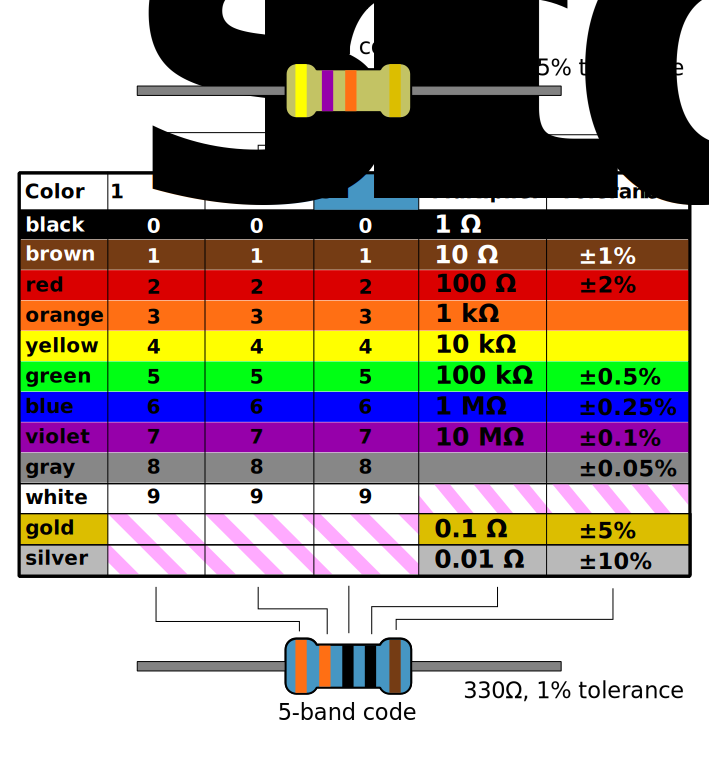
\includegraphics[scale=0.60]{resistorchart.png}
}
\caption{A resistor value color band chart. The `tolerance' stripe (how close the value is guaranteed to be to the stated value) is on the right side. }
\label{fig:resistorchart}
\end{center}
\end{figure}
